\tikzset{every picture/.style={line width=0.75pt}} %set default line width to 0.75pt        

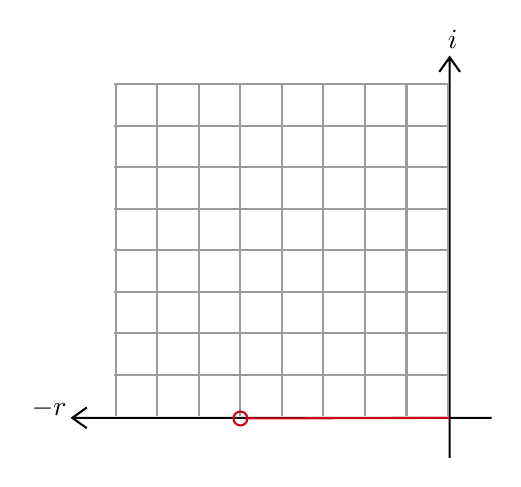
\begin{tikzpicture}[x=0.75pt,y=0.75pt,yscale=-1,xscale=1]
%uncomment if require: \path (0,300); %set diagram left start at 0, and has height of 300

%Shape: Axis 2D [id:dp5907524483347102] 
\draw  (469,209.7) -- (267,209.7)(448.8,36) -- (448.8,229) (274,204.7) -- (267,209.7) -- (274,214.7) (453.8,43) -- (448.8,36) -- (443.8,43)  ;
%Shape: Grid [id:dp6199898397920625] 
\draw  [draw opacity=0] (448,49) -- (287,49) -- (287,209) -- (448,209) -- cycle ; \draw  [color={rgb, 255:red, 155; green, 155; blue, 155 }  ,draw opacity=1 ] (448,49) -- (448,209)(428,49) -- (428,209)(408,49) -- (408,209)(388,49) -- (388,209)(368,49) -- (368,209)(348,49) -- (348,209)(328,49) -- (328,209)(308,49) -- (308,209)(288,49) -- (288,209) ; \draw  [color={rgb, 255:red, 155; green, 155; blue, 155 }  ,draw opacity=1 ] (448,49) -- (287,49)(448,69) -- (287,69)(448,89) -- (287,89)(448,109) -- (287,109)(448,129) -- (287,129)(448,149) -- (287,149)(448,169) -- (287,169)(448,189) -- (287,189) ; \draw  [color={rgb, 255:red, 155; green, 155; blue, 155 }  ,draw opacity=1 ]  ;
%Straight Lines [id:da9323494469903814] 
\draw [color={rgb, 255:red, 208; green, 2; blue, 27 }  ,draw opacity=1 ]   (448.8,209.7) -- (350.35,209.99) ;
\draw [shift={(348,210)}, rotate = 179.83] [color={rgb, 255:red, 208; green, 2; blue, 27 }  ,draw opacity=1 ][line width=0.75]      (0, 0) circle [x radius= 3.35, y radius= 3.35]   ;

% Text Node
\draw (450.23,33) node [anchor=south] [inner sep=0.75pt]    {$i$};
% Text Node
\draw (246,199.4) node [anchor=north west][inner sep=0.75pt]    {$-r$};

\end{tikzpicture}
